\chapter{Odporność na awarie i ataki}

\section{Odporność na awarie i ataki}

W celu zbadania strukturalnej odporności analizowanego grafu WWW przeprowadzono symulacje dwóch typów zaburzeń:
\begin{itemize}
    \item \textbf{Awarie} — losowe usuwanie 10\%, 30\% oraz 50\% wierzchołków.
    \item \textbf{Ataki} — celowe usuwanie 10\%, 30\% oraz 50\% wierzchołków o największym stopniu.
\end{itemize}

Dla każdej modyfikacji przeprowadzono analizę składowych spójności (WCC, SCC, struktura bow-tie), rozkładów stopni, średnich odległości, współczynników klasteryzacji oraz spójności wierzchołkowej.

\subsection{Awaria - usunięcie 10\% losowych wierzchołków}

\begin{itemize}
    \item Wierzchołki: 2710, Krawędzie: 253956
    \item Największa SCC: 1133 wierzchołki
    \item Średnia odległość: 2.67, średnica: 7
    \item Globalna klasteryzacja: 0.697
    \item Spójność wierzchołkowa: 1, punkt artykulacji: \url{https://www.um.edu.mt/}
\end{itemize}

\begin{figure}[H]
\centering
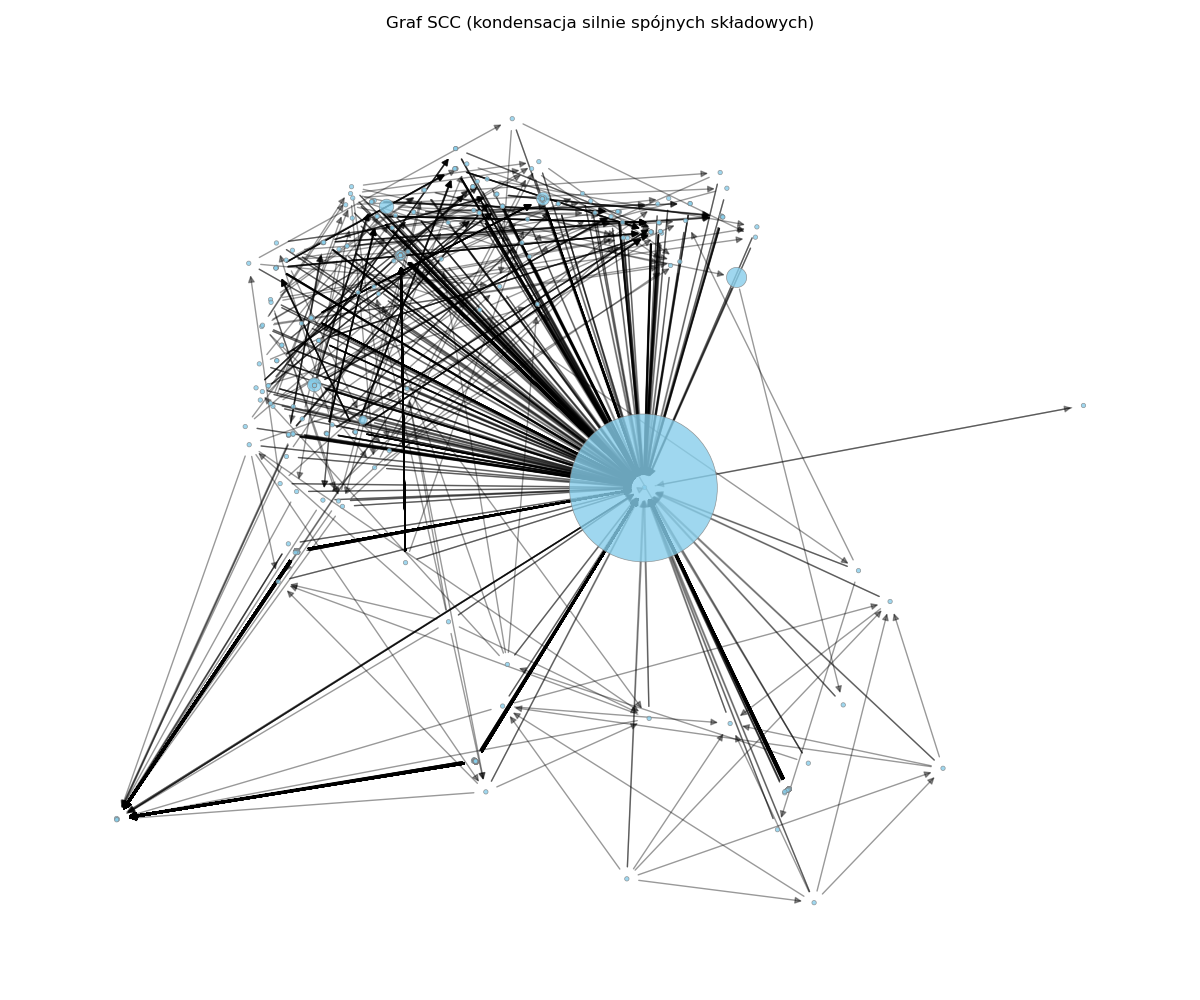
\includegraphics[width=0.45\textwidth]{assets/img_12.png}
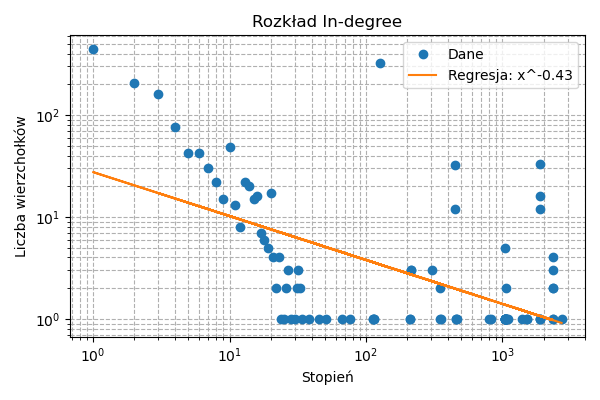
\includegraphics[width=0.45\textwidth]{assets/img_13.png}
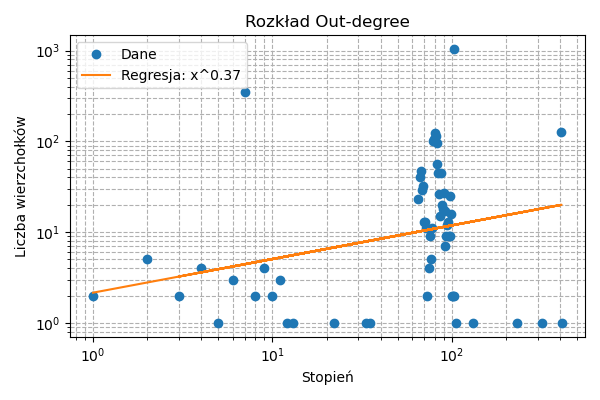
\includegraphics[width=0.45\textwidth]{assets/img_14.png}
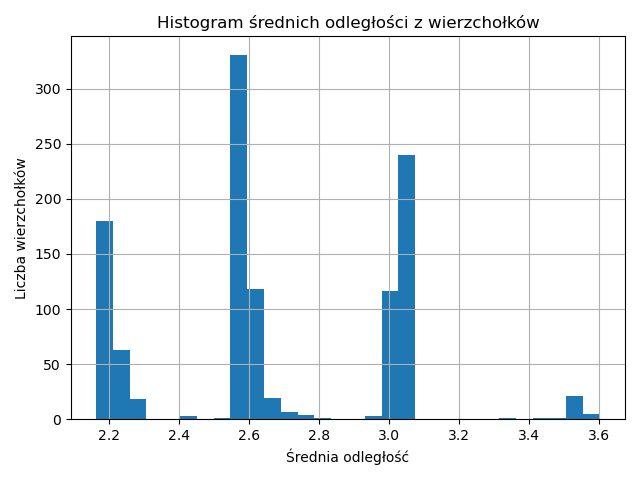
\includegraphics[width=0.45\textwidth]{assets/img_15.png}
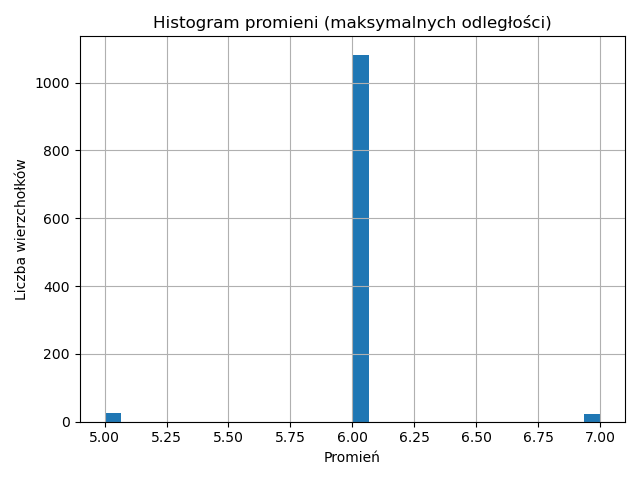
\includegraphics[width=0.45\textwidth]{assets/img_16.png}
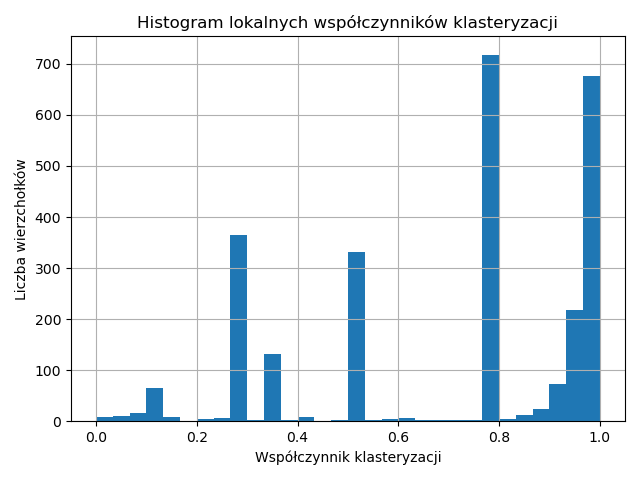
\includegraphics[width=0.45\textwidth]{assets/img_17.png}
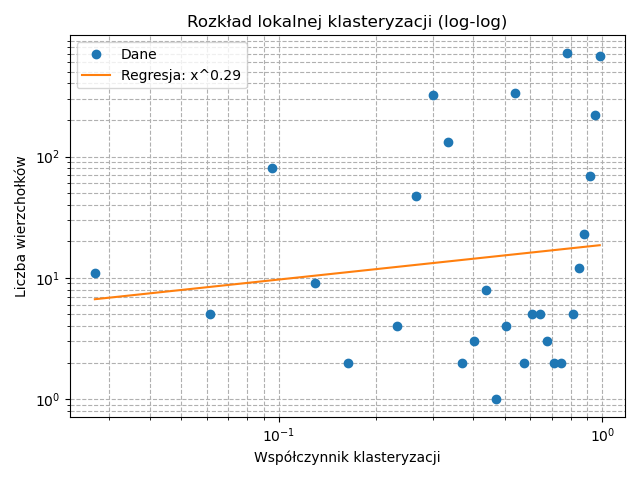
\includegraphics[width=0.45\textwidth]{assets/img_18.png}
\end{figure}

\subsection{Atak - usunięcie 10\% wierzchołków o najwyższym stopniu}

\begin{itemize}
    \item Wierzchołki: 2710, Krawędzie: 10090
    \item Największa SCC: 397 wierzchołków
    \item Średnia odległość: 5.88, średnica: 18
    \item Globalna klasteryzacja: 0.179
    \item Graf niespójny - brak sensu szukać punktów artykulacji
\end{itemize}

\begin{figure}[H]
\centering
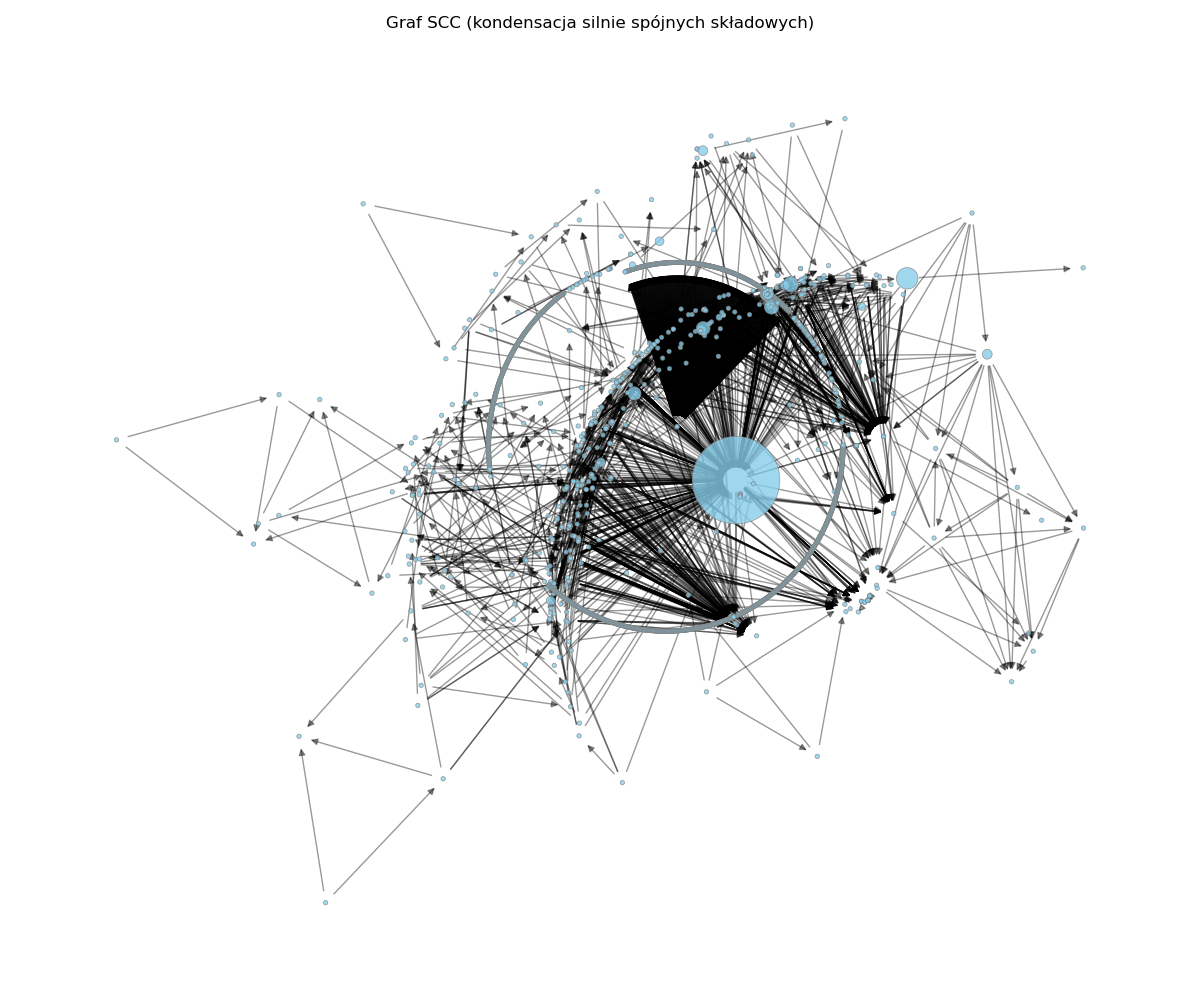
\includegraphics[width=0.45\textwidth]{assets/img_19.png}
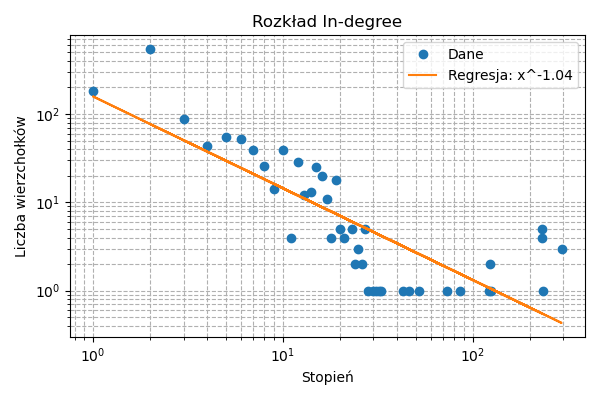
\includegraphics[width=0.45\textwidth]{assets/img_20.png}
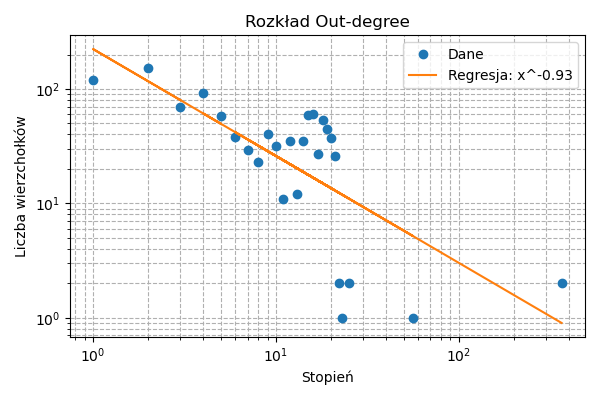
\includegraphics[width=0.45\textwidth]{assets/img_21.png}
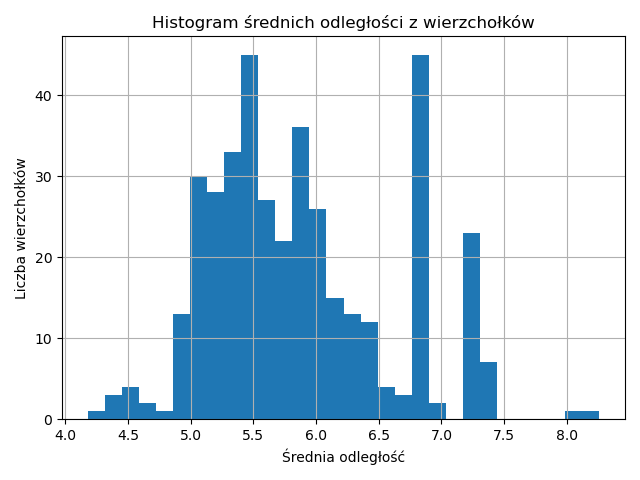
\includegraphics[width=0.45\textwidth]{assets/img_22.png}
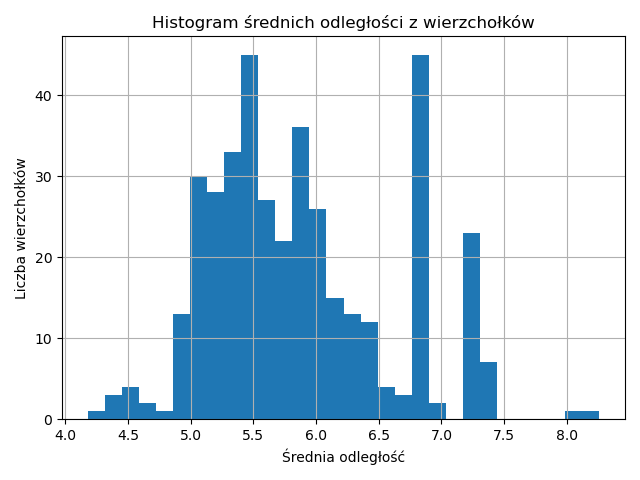
\includegraphics[width=0.45\textwidth]{assets/img_23.png}
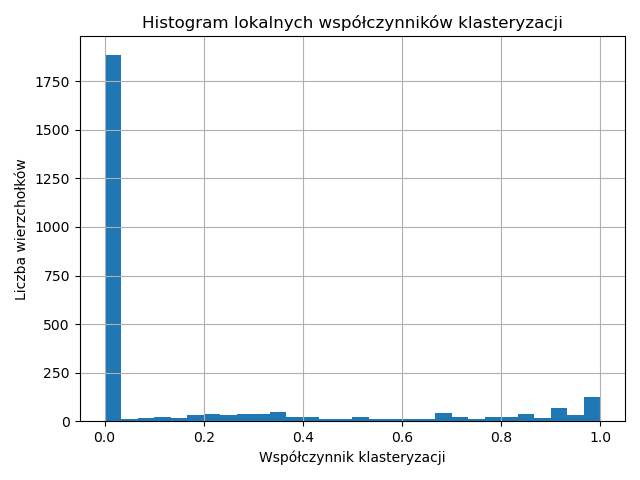
\includegraphics[width=0.45\textwidth]{assets/img_24.png}
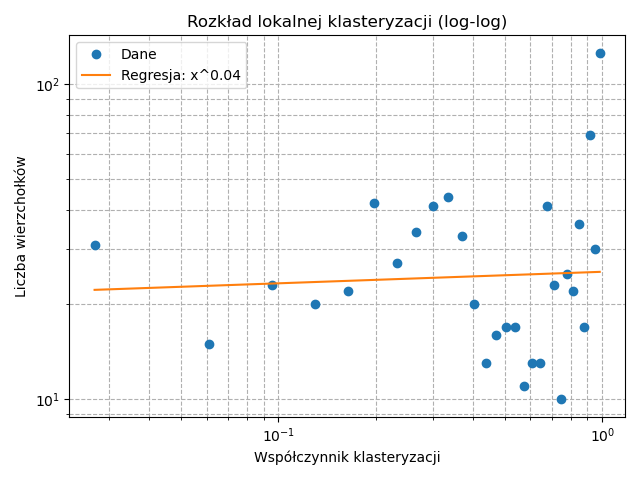
\includegraphics[width=0.45\textwidth]{assets/img_25.png}
\end{figure}

\subsection{Awaria - usunięcie 30\% losowych wierzchołków}

\begin{itemize}
    \item Wierzchołki: 2108, Krawędzie: 159559
    \item Największa SCC: 574
    \item Średnia odległość: 2.63, średnica: 9
    \item Globalna klasteryzacja: 0.721
    \item Punkty artykulacji: \url{https://www.um.edu.mt/}, \url{https://www.um.edu.mt/research/ethics/researchethicsatum/}
\end{itemize}

\begin{figure}[H]
\centering
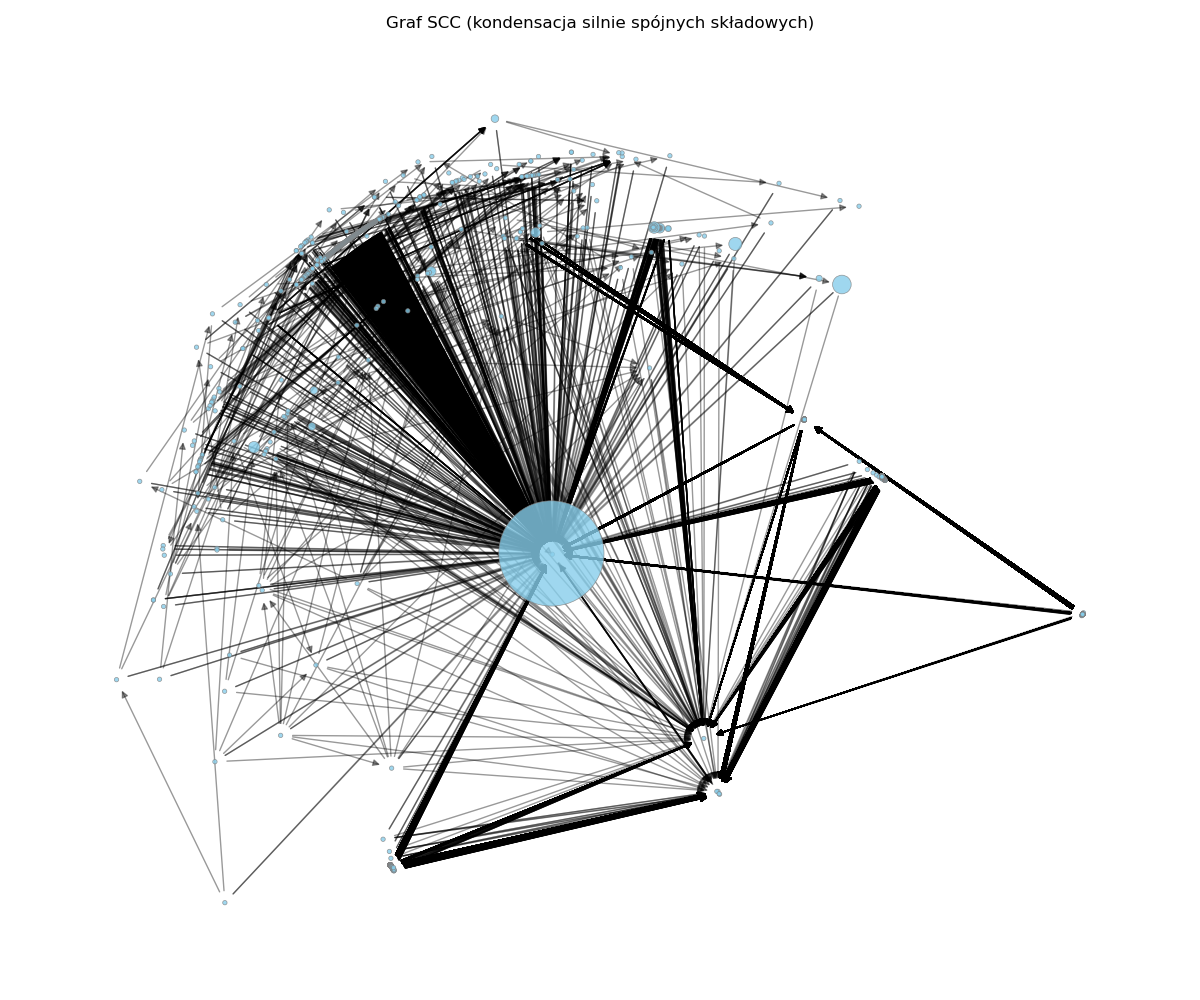
\includegraphics[width=0.45\textwidth]{assets/img_26.png}
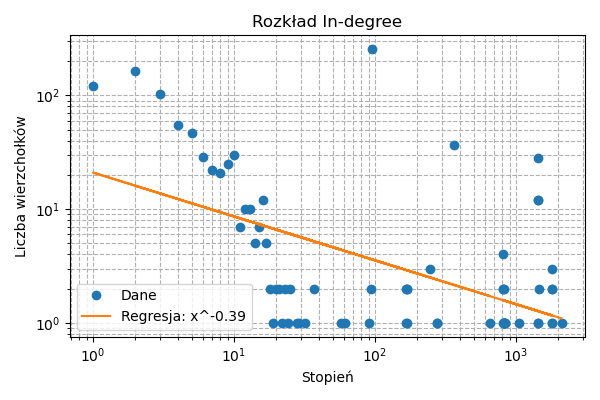
\includegraphics[width=0.45\textwidth]{assets/img_27.png}
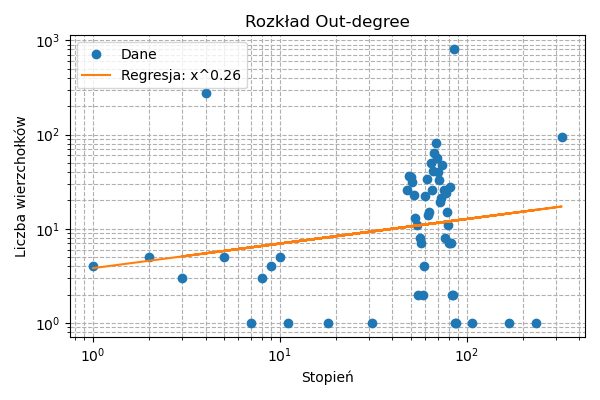
\includegraphics[width=0.45\textwidth]{assets/img_28.png}
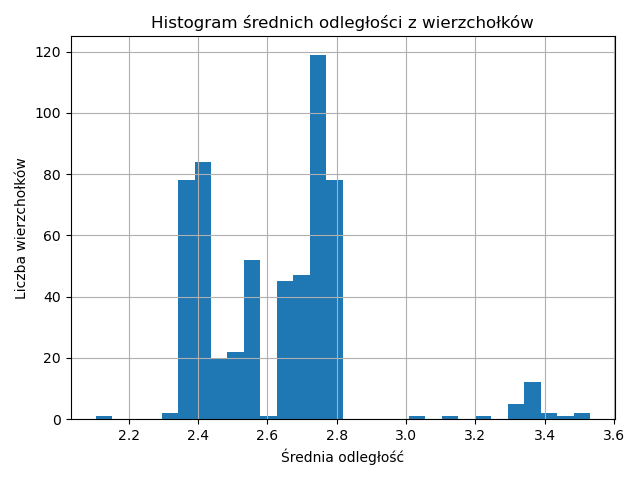
\includegraphics[width=0.45\textwidth]{assets/img_29.png}
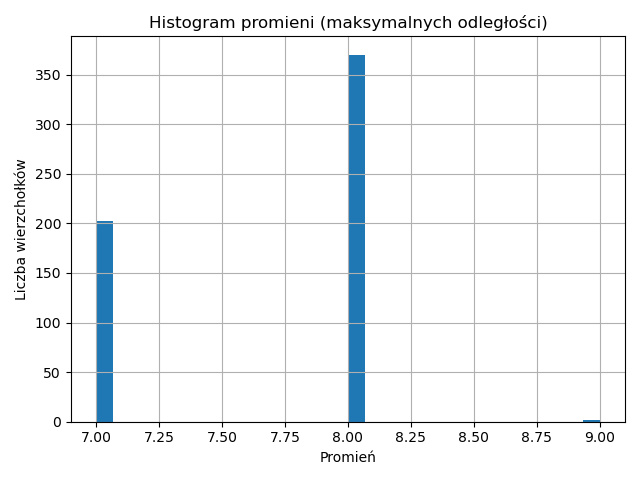
\includegraphics[width=0.45\textwidth]{assets/img_30.png}
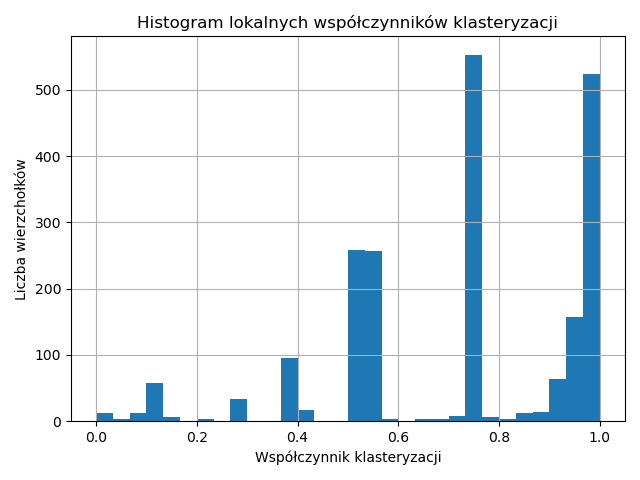
\includegraphics[width=0.45\textwidth]{assets/img_31.png}
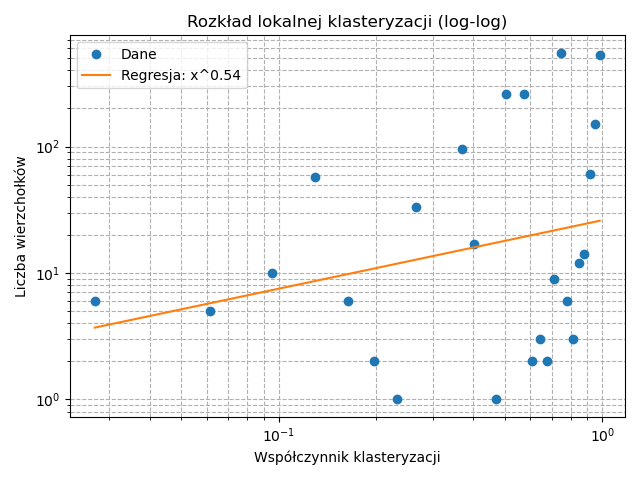
\includegraphics[width=0.45\textwidth]{assets/img_32.png}
\end{figure}

\subsection{Atak - usunięcie 30\% wierzchołków o najwyższym stopniu}

\begin{itemize}
    \item Wierzchołki: 2108, Krawędzie: 3014
    \item Największa SCC: 85
    \item Średnia odległość: 5.26, średnica: 17
    \item Globalna klasteryzacja: 0.1757
    \item Graf niespójny - brak sensu szukać punktów artykulacji
\end{itemize}

\begin{figure}[H]
\centering
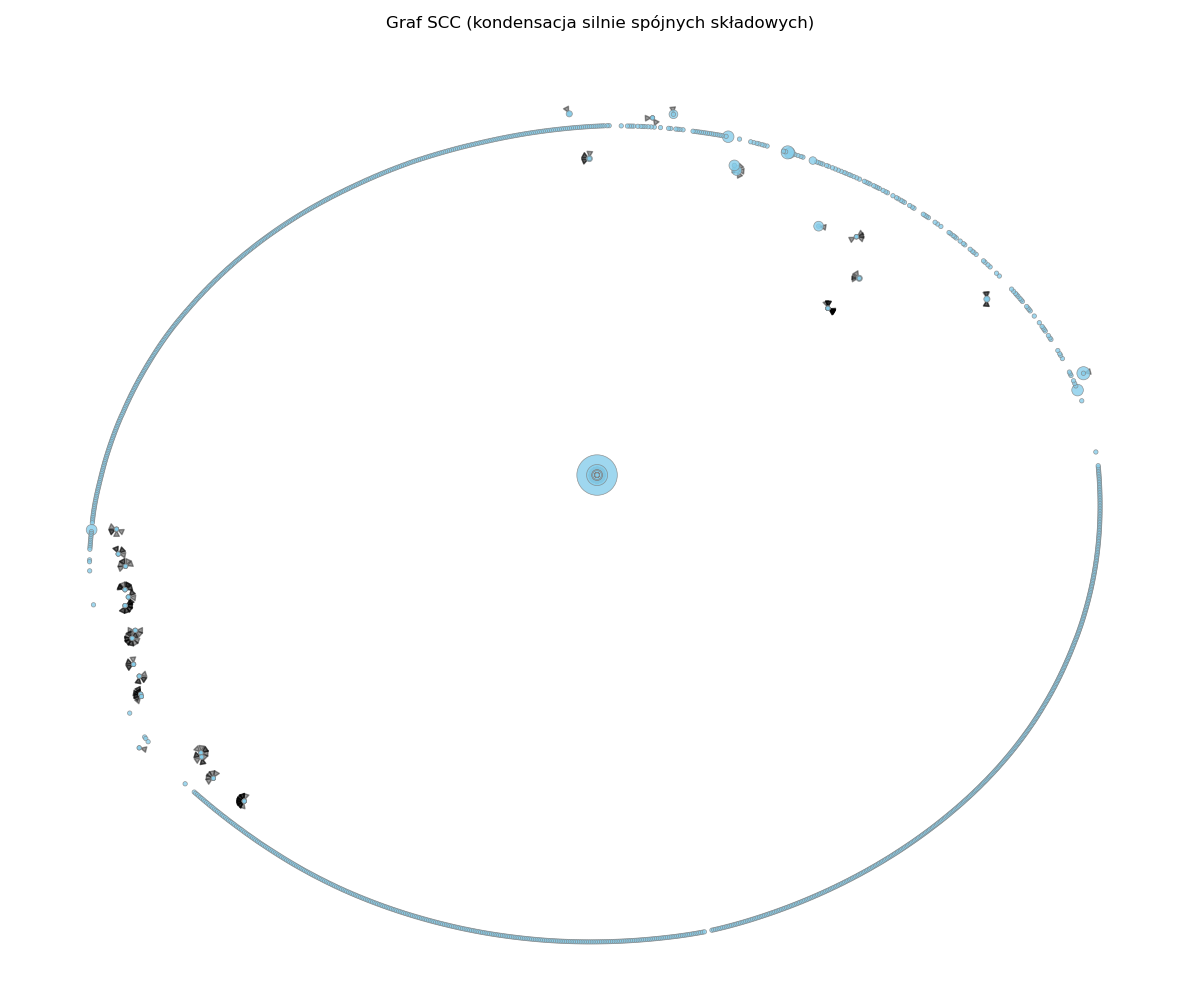
\includegraphics[width=0.45\textwidth]{assets/img_33.png}
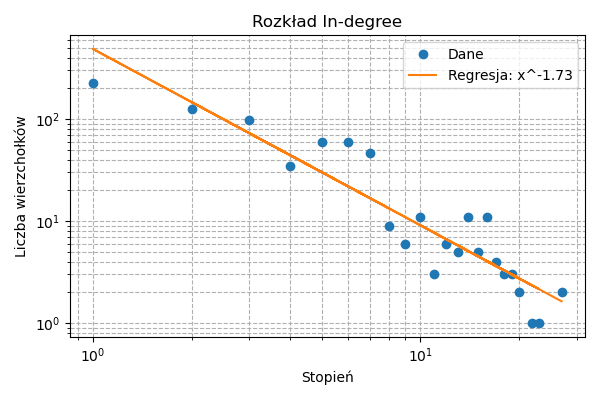
\includegraphics[width=0.45\textwidth]{assets/img_34.png}
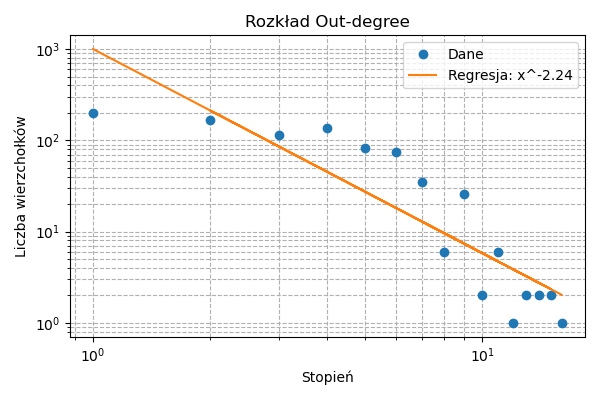
\includegraphics[width=0.45\textwidth]{assets/img_35.png}
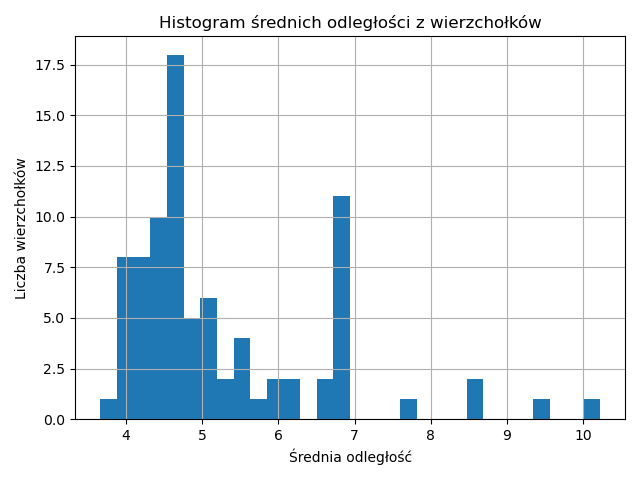
\includegraphics[width=0.45\textwidth]{assets/img_36.png}
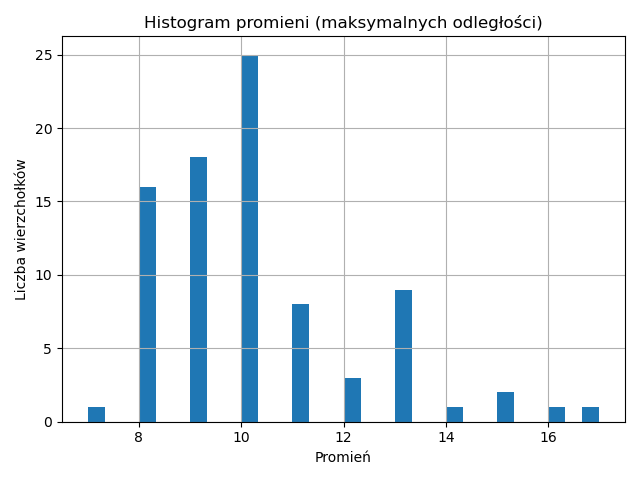
\includegraphics[width=0.45\textwidth]{assets/img_37.png}
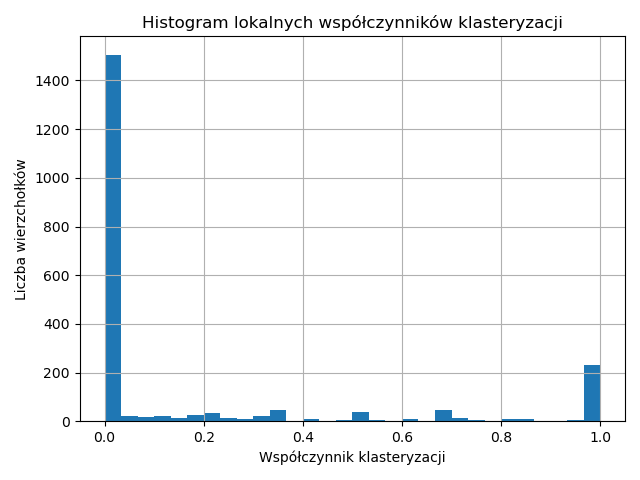
\includegraphics[width=0.45\textwidth]{assets/img_38.png}
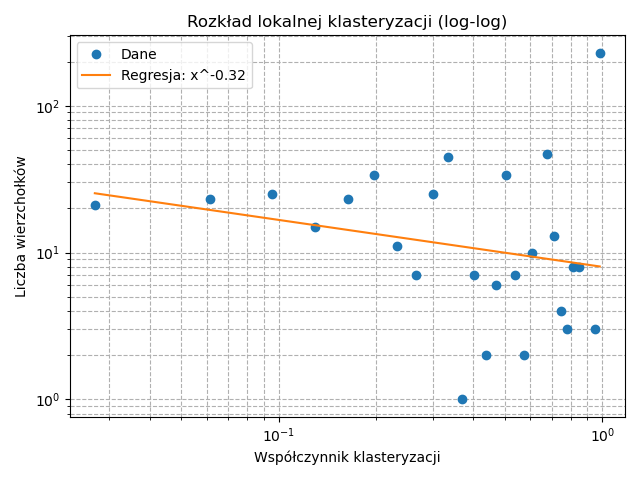
\includegraphics[width=0.45\textwidth]{assets/img_39.png}
\end{figure}

\subsection{Awaria - usunięcie 50\% losowych wierzchołków}

\begin{itemize}
    \item Wierzchołki: 1506, Krawędzie: 72649
    \item Największa SCC: 573
    \item Średnia odległość: 2.73, średnica: 6
    \item Globalna klasteryzacja: 0.6195
    \item Punkty artykulacji: 2 (jak wcześniej)
\end{itemize}

\begin{figure}[H]
\centering
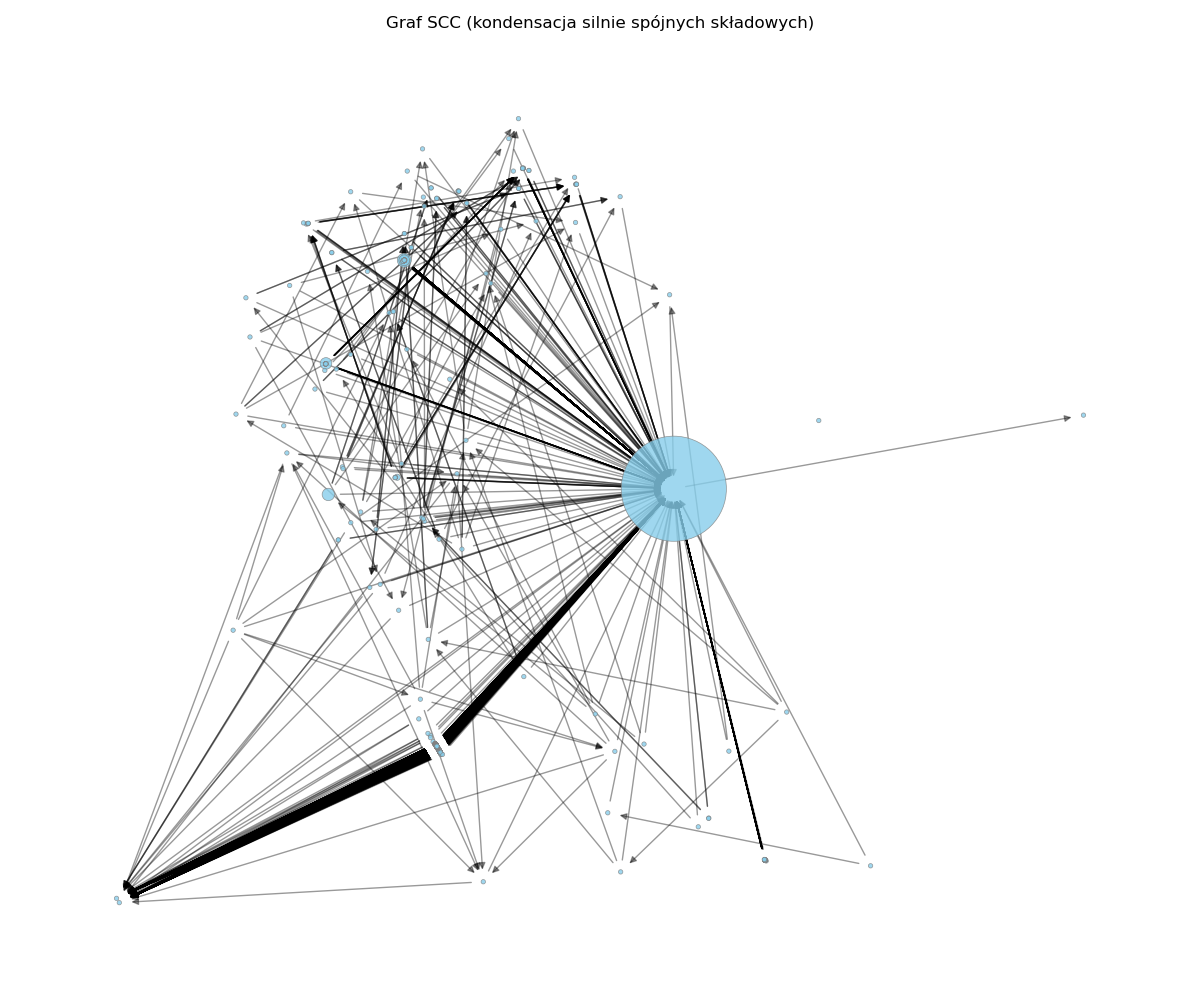
\includegraphics[width=0.45\textwidth]{assets/img_40.png}
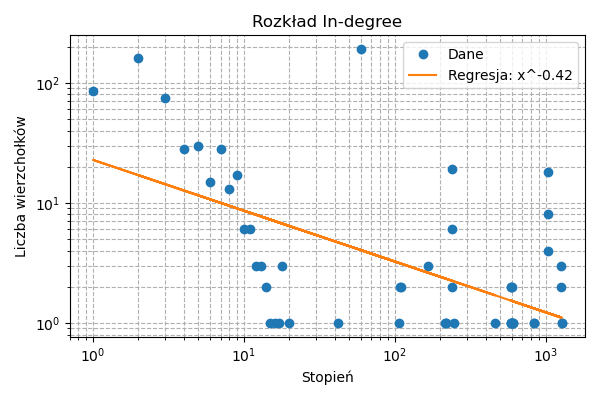
\includegraphics[width=0.45\textwidth]{assets/img_41.png}
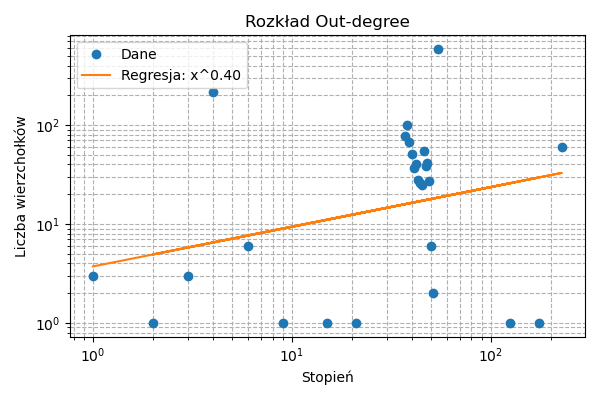
\includegraphics[width=0.45\textwidth]{assets/img_42.png}
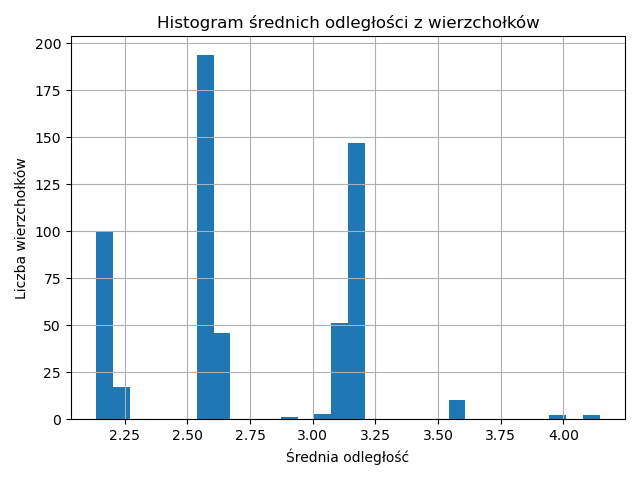
\includegraphics[width=0.45\textwidth]{assets/img_43.png}
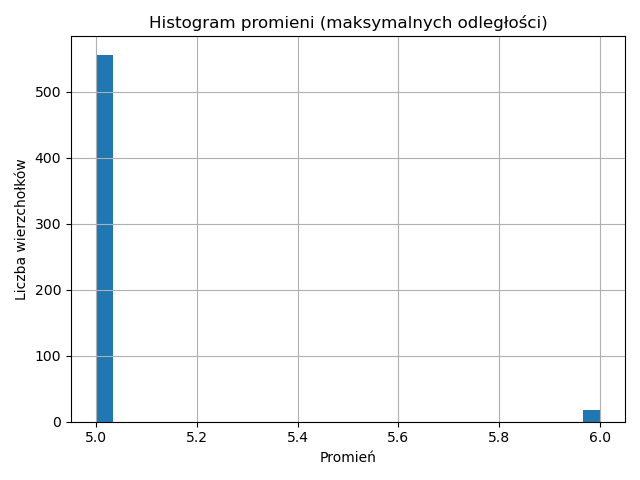
\includegraphics[width=0.45\textwidth]{assets/img_44.png}
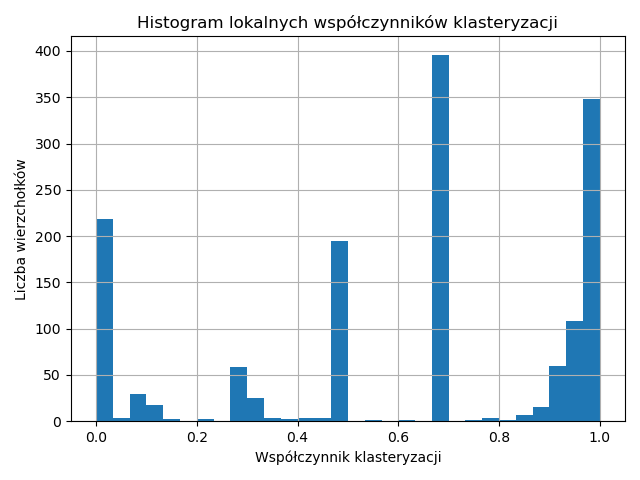
\includegraphics[width=0.45\textwidth]{assets/img_45.png}
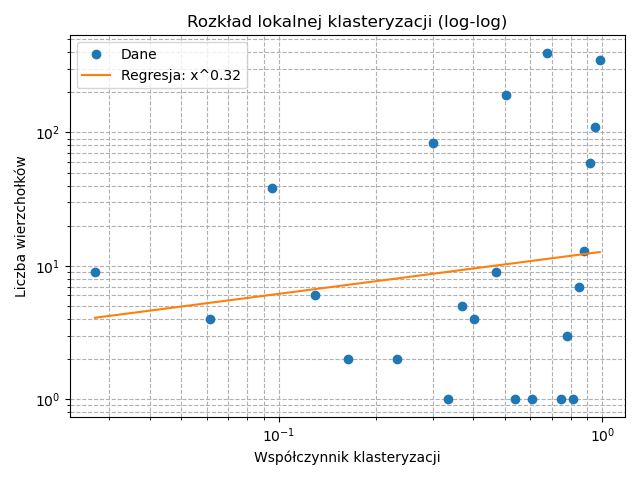
\includegraphics[width=0.45\textwidth]{assets/img_46.png}
\end{figure}

\subsection{Atak - usunięcie 50\% wierzchołków o najwyższym stopniu}

\begin{itemize}
    \item Wierzchołki: 1506, Krawędzie: 3014
    \item Największa SCC: 85
    \item Średnia odległość: 5.26, średnica: 17
    \item Globalna klasteryzacja: 0.2460
    \item Graf niespójny
\end{itemize}

\begin{figure}[H]
\centering
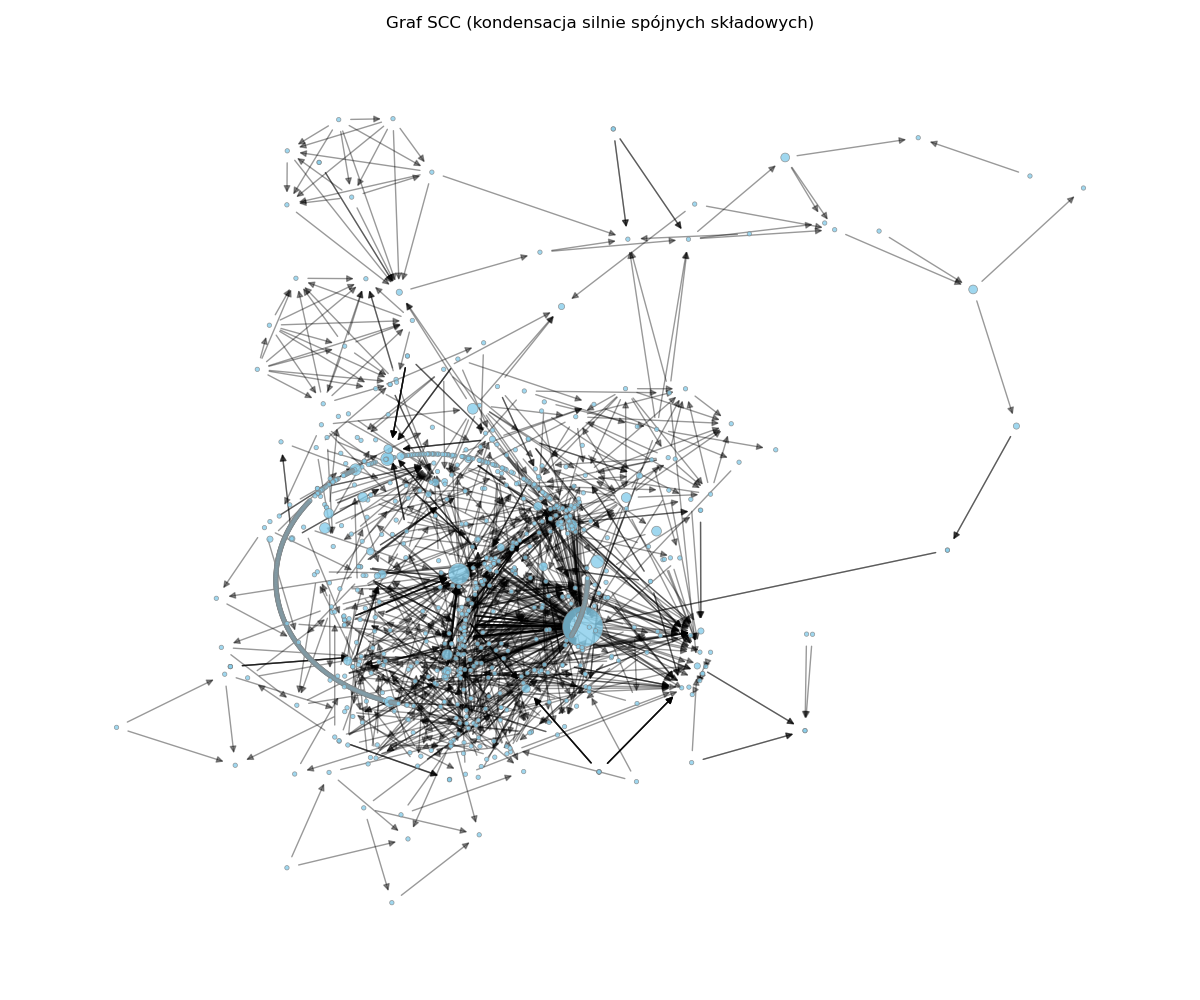
\includegraphics[width=0.45\textwidth]{assets/img_47.png}
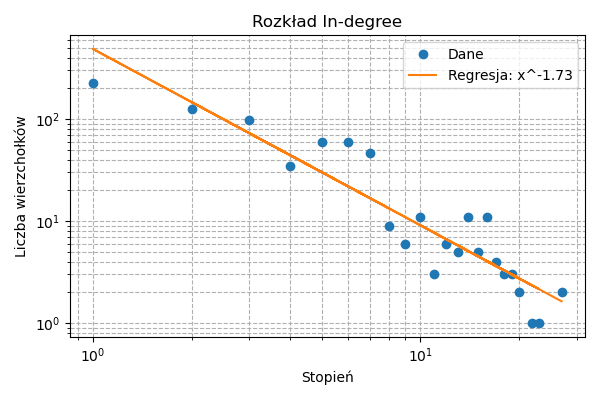
\includegraphics[width=0.45\textwidth]{assets/img_48.png}
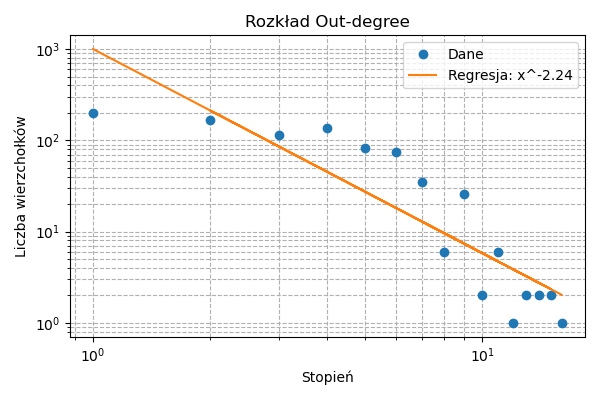
\includegraphics[width=0.45\textwidth]{assets/img_49.png}
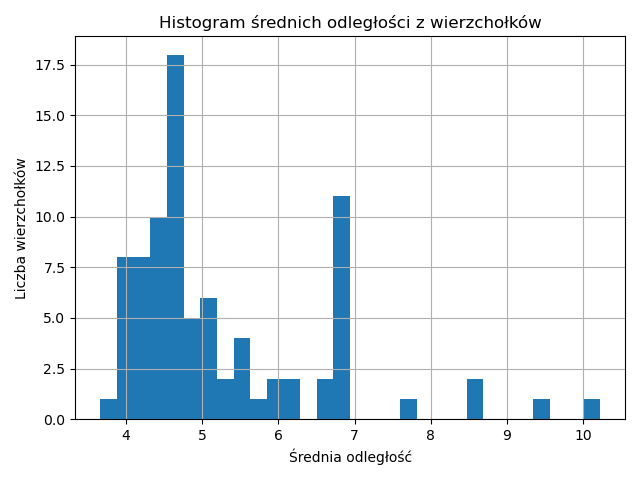
\includegraphics[width=0.45\textwidth]{assets/img_50.png}
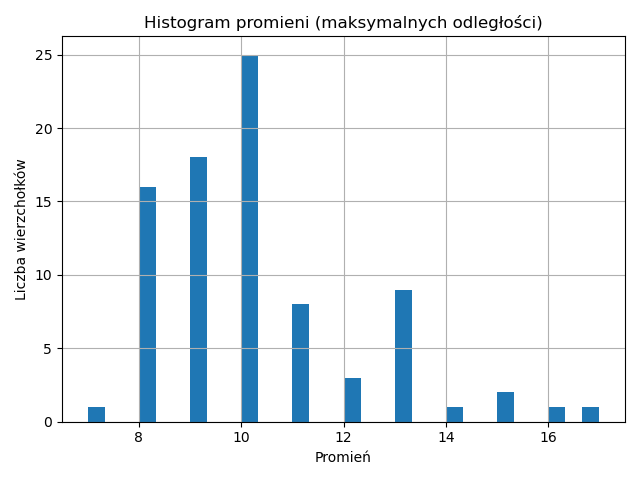
\includegraphics[width=0.45\textwidth]{assets/img_51.png}
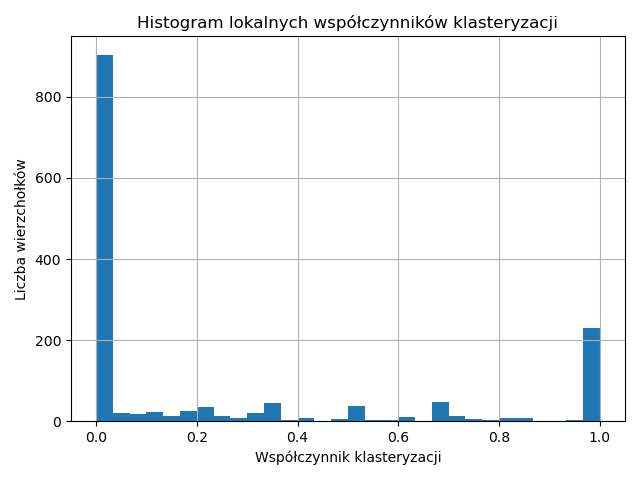
\includegraphics[width=0.45\textwidth]{assets/img_52.png}
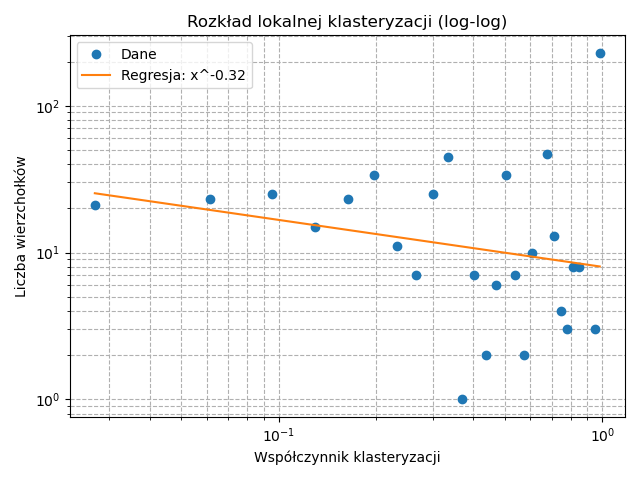
\includegraphics[width=0.45\textwidth]{assets/img_53.png}
\end{figure}

\subsection{Podsumowanie}

Wyniki symulacji wskazują na istotne różnice w zachowaniu grafu w zależności od typu zakłócenia (awaria losowa vs atak ukierunkowany). Poniżej przedstawiono szczegółowe wnioski:

\subsubsection{Składowe spójności}

\begin{itemize}
    \item \textbf{Awarie losowe} nie naruszają znacząco struktury spójności:
    \begin{itemize}
        \item nawet przy 50\% usuniętych wierzchołków liczba WCC = 2,
        \item największa SCC pozostaje względnie duża (573 wierzchołków),
        \item struktura typu bow-tie zostaje zachowana (IN/OUT obecne, TENDRILS minimalne).
    \end{itemize}

    \item \textbf{Ataki} natomiast:
    \begin{itemize}
        \item szybko rozbijają graf (np. już przy 10\% - ponad 1200 WCC),
        \item SCC staje się bardzo mała (np. tylko 85 wierzchołków przy 30-50\%),
        \item rośnie liczba wysp i tendrili (ponad 1000 dla 50\%),
        \item graf traci strukturę rdzeniową - IN/OUT stają się słabo połączone z SCC.
    \end{itemize}
\end{itemize}

\subsubsection{Rozkłady stopni}

\begin{itemize}
    \item Rozkłady stopni przy awariach zachowują wcześniejsze właściwości — wykładniki potęgowe są bliskie 0.4 (niskie R² $\approx$ 0.3-0.4), co sugeruje niewielką zmianę struktury lokalnej.

    \item W przypadku ataków, rozkłady te ulegają znacznej zmianie:
    \begin{itemize}
        \item wykładniki in-degree/out-degree spadają do wartości poniżej $-1.7$,
        \item współczynniki determinacji $R^2$ osiągają nawet 0.85,
        \item co oznacza, że usunięcie hubów „ujawnia” potęgową strukturę grafu.
    \end{itemize}
\end{itemize}

\subsubsection{Odległości i średnice}

\begin{itemize}
    \item Przy awariach średnie odległości pozostają stabilne (2.6-2.7), a średnice nie przekraczają 9 — co sugeruje zachowanie efektu małego świata.
    \item Po atakach średnie odległości wzrastają dramatycznie do ponad 5, a średnice sięgają 17-18 — sieć staje się wyraźnie mniej efektywna informacyjnie.
\end{itemize}

\subsubsection{Klasteryzacja}

\begin{itemize}
    \item Globalny współczynnik klasteryzacji utrzymuje się na poziomie $\sim$0.7 dla awarii.
    \item W przypadku ataków spada do $\sim$0.17-0.24, co świadczy o zerwaniu lokalnych struktur spójnych.
\end{itemize}

\subsubsection{Spójność wierzchołkowa}

\begin{itemize}
    \item Dla awarii, graf pozostaje 1-spójny — nadal występują punkty artykulacji.
    \item Dla ataków graf ulega dezintegracji, co uniemożliwia analizę rozspajających wierzchołków (graf nie jest już spójny).
\end{itemize}

\subsubsection{Wniosek końcowy}

\textbf{Graf sieci WWW uczelni ma klasyczne właściwości sieci skali bezwzględnej (scale-free)} — jest:
\begin{itemize}
    \item \textbf{odporny na awarie} — przypadkowe usunięcia nie zakłócają znacząco funkcjonowania,
    \item \textbf{podatny na ataki} — usunięcie stron centralnych (o najwyższym stopniu) powoduje szybkie rozbicie całej struktury.
\end{itemize}

Z punktu widzenia zarządzania infrastrukturą informacyjną, oznacza to konieczność zapewnienia nadmiarowości i kopii zapasowych dla węzłów centralnych (np. strona główna, główne katalogi).
